% This is samplepaper.tex, a sample chapter demonstrating the
% LLNCS macro package for Springer Computer Science proceedings;
% Version 2.20 of 2017/10/04
%
\documentclass[runningheads]{llncs}
%
\usepackage{wrapfig}
\usepackage{graphicx}
\usepackage{booktabs} % For formal tables
\usepackage{minted}
\usepackage{multirow}
\usepackage{graphicx}
\usepackage{subcaption}
\usepackage{amssymb}
\usepackage{amsmath}
\captionsetup{compatibility=false}
\usepackage{hyperref}
% Used for displaying a sample figure. If possible, figure files should
% be included in EPS format.
%
% If you use the hyperref package, please uncomment the following line
% to display URLs in blue roman font according to Springer's eBook style:
% \renewcommand\UrlFont{\color{blue}\rmfamily}

\begin{document}
%
\title{BTestBox - A tool for testing B translators and coverage of B models}
%
%\titlerunning{Abbreviated paper title}
% If the paper title is too long for the running head, you can set
% an abbreviated paper title here
%
\author{Diego de Azevedo Oliveira \inst{1} \and %\orcidID{0000-1111-2222-3333} \and
Val{\'e}rio Medeiros Jr\inst{2}\orcidID{0000-0001-6255-5026} \and
David D{\'e}harbe\inst{3}\and %\orcidID{2222--3333-4444-5555} \and
Martin A. Musicante \inst{4}\orcidID{0000-0001-5589-3895}
}
%
\authorrunning{D. Azevedo et al.}
% First names are abbreviated in the running head.
% If there are more than two authors, 'et al.' is used.

\institute{Université de Sherbrooke, Canada\\
\email{diegodeazevedooliveira@gmail.com}
\and
Instituto Federal de Educa{\c c}{\~a}o, Ci{\^e}ncia e Tecnologia do Rio Grande do Norte, Brazil\\
\email{valerio.medeiros@ifrn.edu.br} \and
Clearsy System Engineering, France\\
\email{david.deharbe@clearsy.com}
\and
Universidade Federal do Rio Grande do Norte, Brazil\\
\email{mam@dimap.ufrn.br}}

%\institute{Université de Sherbrooke, Canada \and
%Springer Heidelberg, Tiergartenstr. 17, 69121 Heidelberg, Germany
%\email{lncs@springer.com}\\
%\url{http://www.springer.com/gp/computer-science/lncs} \and
%ABC Institute, Rupert-Karls-University Heidelberg, Heidelberg, Germany\\
%\email{\{abc,lncs\}@uni-heidelberg.de}}
%\end{comment}


%
\maketitle              % typeset the header of the contribution
%
\begin{abstract}
Formal software design processes based on refinement include steps
such as source code analysis and code generation, which are usually
out of the scope of the formal argument of correctness.
To mitigate the risk of introducing errors in these phases,
certifications of regulation entities demand or recommend testing the
generated software, using some code coverage criteria (e.g., MC/DC
coverage for DO-178C, which is well demanded in the aeronautical
industry).
We propose improvements over BTestBox, a tool for automatic generation
of tests for software components developed with the B method.
BTestBox supports several code coverage criteria and applies to code
generators for different languages.
The tool uses a constraint solver to produce tests, being able to
identify dead code and tautological branching conditions.
It also generates reports with different metrics and may be used as an
extension to the Atelier B (an IDE developed by ClearSy, used to write
software for critical safety systems).
Our tool performs a double task: first, it acts on the B model, by
checking code coverage.
In a second moment, the tool performs the translation of lower level B
specifications into programming language code, runs tests and compares
their results with the expected output of the test cases.
The present version of BTestBox uses parallelization techniques that
significantly improve its performance.
The results presented here are encouraging, showing performance
numbers that are one order of magnitude better than for the previous
version of the tool.

%\keywords{First keyword  \and Second keyword \and Another keyword.}
\keywords{Proofs, Model-based testing, Code coverage.}
\end{abstract}
%
%
%


\section{Introduction}

Creating software using the B method \cite{abrial2005b} follows a production flow that goes from an abstract model to the code translated into the target language. 
%Compatible compilers used to translate the code are not dependable, compilers' errors may silently introduce bugs from correct source code \cite{leroy2009formal}.
Since the compatible compilers used to translate the code are not dependable, compiler errors may silently introduce bugs from the correct source code \cite{leroy2009formal}.
Thus, BTestBox is being developed as a solution to test the translated code and to assure that the translation is performed well. \textcolor{blue}{Additionally, it may help the verification process to find counterexamples.}
Model-based testing (MBT) provides an approach for the automatic
generation of test cases from models \cite{dalal1999model}. The proposed tool uses MBT and seeks to satisfy code coverage criteria.

%Using a formal method as B is one technique to guarantee the specification behaviour as the user wants.
Using a formal method such as B is a technique to assure the behaviour of a specification.
Thus, this method has been used for many researches, over many years, in the development of critical systems \cite{valerio_thesis:2016}. B is based on the Dijkstra notes \cite{dijkstra1976discipline}; it uses the generalised substitution theory \cite{hoare2002proof} and the abstract machine notation. It supports a modular modelling:  every component has its own specified module with different levels of abstraction, starting with an abstract machine and with sub-sequential modelling, until a concrete implementation. The goal is to have a proven implementation. However, the B code needs to be translated into binary code. \textcolor{blue}{This process can lead to errors and requires more attention}. The B process is demonstrated in Figure \ref{fig:Bmethod}.

\begin{figure*}[ht]
    \centering
    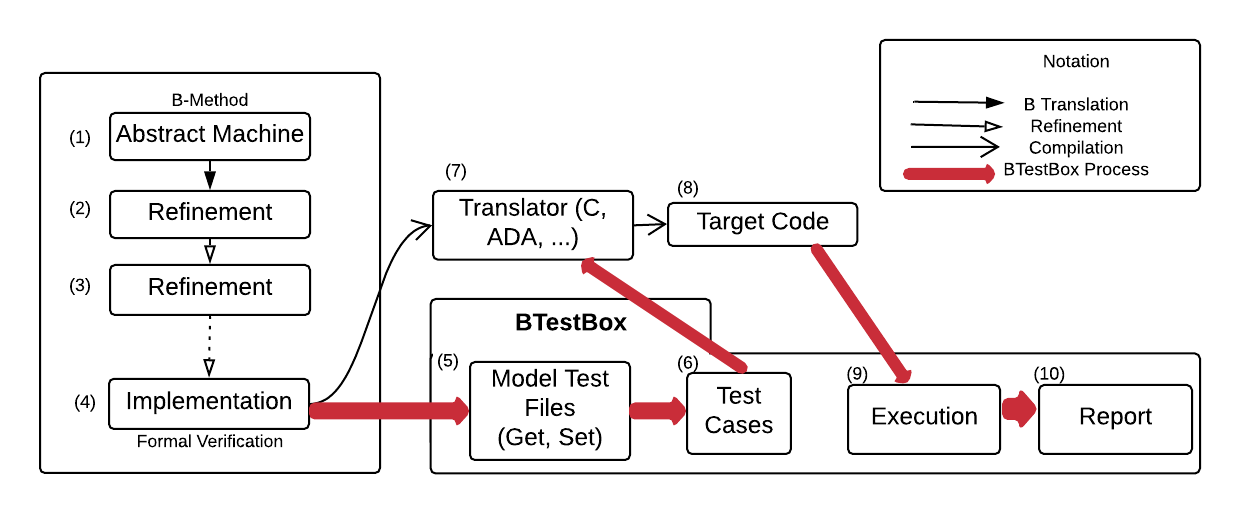
\includegraphics[width = \textwidth,natwidth=1240,natheight=513]{imagens/BMethodBTestBoxColor.png}
    \caption{Overview of the B process with the BTestBox process.}
    \label{fig:Bmethod}
\end{figure*}

Translators are used to perform the conversion from B representation to another computer language such as C, ADA, and LLVM. Each translator can translate a subset of B, called B0. Moreover, a translator can have specific restrictions. %Such restrictions are not well documented and may confuse the user. 
Additionally, compilers can insert bugs even with the correct source code \cite{leroy2009formal}, and the code generators used with B demand additional safety criteria because they are employed in critical systems.

Testing techniques may supplement formal methods during the verification and validation process. They are used for an in-depth verification of the system. The formal methods are limited, and the use of software testing can quickly identify failures and expose defects introduced during the development of the concrete phase or the maintenance of the code \cite{ernesto_thesis:2016}. Also, some certificates such as DO-178B, required by the Federal Aviation Administration (FAA), demand the use of software testing and measuring coverage over the code.

The BTestBox may be used as an Atelier-B extension and, from its interface, can automatically test B specifications. Our tool - BTestBox - receives, as input, a B implementation, the target translator (and profile needed for it to run), one compiler, one coverage criterion, the folder project, and the logic expression solver (ProB)\footnote{ProB is an animator, constraint solver and model checker for B models \cite{1_leuschel_2017}.} directory. Then, the BTestBox generates the test cases to cover the criterion in B, so that the models are translated and executed in the target language. Next, they are compared with the expected values and finally reported. In Figure \ref{fig:Bmethod} it is possible to observe where our tool fits in the B process.

In the current state, BTestBox is fully automatic and capable of testing translations from B implementations to C, thus indicating if there is an error in the translation and reporting the coverage rate for the following criteria: Statement Coverage, Clause Coverage, Path Coverage, Branch Coverage, and Combinatorial Coverage. 
%Each coverage has its functionality such as: identifying dead code with Code Coverage; logic tautology with functional coverages (Path and Branch coverage); and analysing the program flow with different logic decisions (Clause Coverage and MC/DC). 
The tool and the results of an evaluation with the B language are presented in this paper. The contributions of BTestBox are the following:




\begin{itemize}
    \item Avoiding the waste of time with the construction of manual test cases by supplying a full automatic model-based process for generation of executable supported criteria test cases for B implementations.% \textcolor{red}{ }
    %Ajudar no processo de verificação, pois ajudar a encontrar contra exemplos de entrada na especificação.
    \item Verifying the correctness of the B compiler while testing the translated code developed with the B formal method process using the supported criteria test cases consequently, it helps to find dead code and unnecessary conditions.
    %Consequentemente isso ajuda a encontrar código morto, codições desnecessárias
\end{itemize}

This article is organised as follows: %Section \ref{sec:BMethod} gives a brief terminology used in our work. 
Section \ref{sec:BTestBox} explains the BTestBox methodology, the background needed to understand the BTestBox process, how the tool works, and how it is associated with the B method. Section \ref{sec:Results} shows the results, metrics, threats, and limitations of our tool. Section \ref{sec:RelatedWork} describes the related work. Section \ref{sec:Conclusion} presents the conclusions and the future work.

\section{Methodology} \label{sec:BTestBox}

In this section, we present the BTestBox methodology and the background needed to understand the process. Our tool tries to confirm the reliability of the B translator while executing the translated code with generated test cases to verify one coverage criterion. To accomplish this objective, BTestBox takes one B implementation and tries to find test cases where one coverage criterion, chosen by the user, shall be achieved. To create the test cases, BTestBox draws the execution flow of a given implementation and uses Hoare's Logic to write a predicate which comprises the possible values for running a path of the flow. Then, it is evaluated and, if one possible solution is found, the values of the input and output will be stored. The creation of test cases continues until the execution of the paths achieves the coverage criteria or until all the paths generated a test case and the criteria was not achieved. Our tool prepares components capable of executing and checking the execution of the test cases after the translation. Finally, the test components are translated and executed, and the metrics are reported.

\subsection{Path Generation}

This section describes how BTestBox identifies the paths from a given B implementation. It is based on directed graphs and takes advantage of the B method properties. From the graph definition:

\begin{itemize}
    \item An \textit{N} set of nodes.
    \item An $N_0$ set of initial nodes, where $N_0 \subseteq N$.
    \item An $N_f$ set of final nodes, where $N_f \subseteq N$.
    \item An E set of edges, where E is a subset of $N \times N$.
\end{itemize}

Since the operations in B can only have one origin and has an end declaration. The initial and final set nodes of the graph for a given B operation are unitary test sets.

Edges are elements that go from one node and reach the other and are written as ($n_i$,$n_j$). This demonstrates that the edge connects the $n_i$ node to $n_j$.

A path of a graph G is a sequence of nodes [$n_1$,$n_2$,\ldots,$n_M$], in which each adjacent pair of nodes ($n_i$, $n_{(i+1)}$), $1 \leq i < M$ is found at the $E$ set of edges.

For some coverage criteria, it is required that the graph starts at one node and finishes at the other. This is only possible if the nodes are connected by a path. When these coverage criteria are applied in specific graphs, they may produce paths that are impossible to execute. With our tool and the coverage criteria supported by the BTestBox, we can identify these paths and recognise the user's dead codes or useless guard clauses. At the moment, BTestBox supports the following criteria:

\begin{itemize}
    \item Statement Coverage (ST): Criterion in which every command of the code shall be executed at least once \cite{ammann2008introduction}.
    \item Branch Coverage (BC): To achieve this criterion, it is necessary to reach every branch in the control flow graph \cite{ammann2008introduction}.
    \item Path Coverage (PC): It is necessary to reach all different paths in the control flow graph to achieve this coverage \cite{ammann2008introduction}.
    \item Clause Coverage (CC): Given a predicate, each clause inside the predicate needs to be evaluated as either true or false at least once \cite{ammann2003coverage}.
    \item Combinatorial Coverage (CoC): Given a predicate, each possible combination of the clauses shall be evaluated \cite{ammann2003coverage}.
\end{itemize}

Generating a graph and the number of paths does not depend on which coverage criteria is chosen, but the number of paths needed to be executed depends on the coverage. Given the B implementation found in Figure \ref{fig:russianMultImp} and its ``RussMult'' operation, BTestBox can draw the graph shown in Figure \ref{fig:russianMultGraph}.

% \begin{figure}[ht]
%         \centering
%         \begin{minipage}{0.58\textwidth}
%             \centering
        
%             \begin{minted}[escapeinside=||,mathescape=true,frame=single,firstnumber=1,linenos=false,breaklines,fontsize=\small]{ocaml}
% IMPLEMENTATION RussianMult_i
% REFINES RussianMult
% CONCRETE_VARIABLES  xx, yy, total
% INVARIANT  xx |$\in$| |$\mathbb{N}$| |$\wedge$| yy |$\in$| |$\mathbb{N}$| |$\wedge$| total |$\in$| |$\mathbb{N}$|
% INITIALISATION xx, yy, total := 0, 0, 0
% OPERATIONS
%   RussMult(aa,bb) = 
%     xx := aa; yy := bb; total := 0;
%     WHILE xx > 0 DO
%       IF xx mod 2 = 1 THEN total := total + yy END;
%       xx := xx / 2; yy := yy * 2
%     INVARIANT xx |$\in$| |$\mathbb{N}$| |$\wedge$| total + xx * yy = aa * bb
%     VARIANT xx
%     END
%   END
% END
%                 \end{minted}
%         \caption{Implementation of Russian multiplication. \cite{schneider2001b}}
%         \label{fig:russianMultImp}
%     \end{minipage}%
% \end{figure}

% \begin{figure}[ht]
% \centering
% 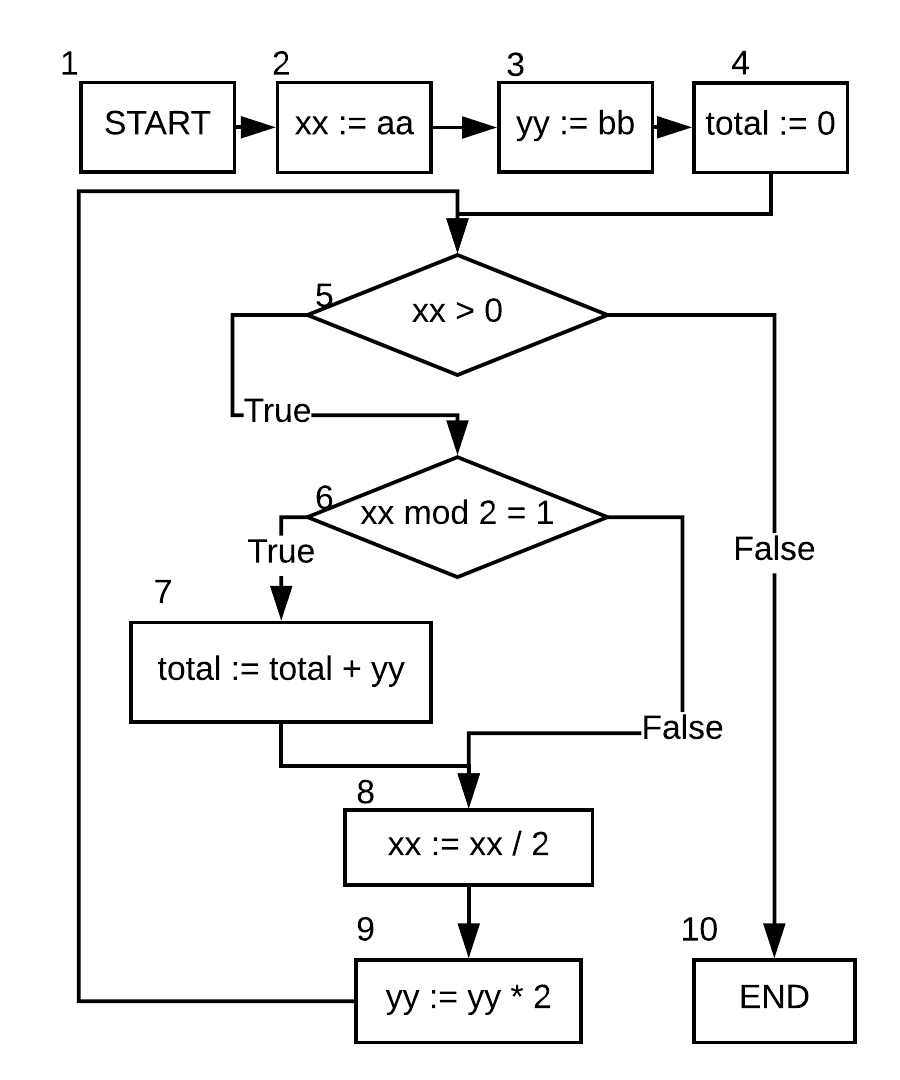
\includegraphics[width=0.45\textwidth]{imagens/lacoGrafo.png}
% \caption{Graph of the operation ``RussMult''.}
% \label{fig:russianMultGraph}
% \end{figure}

\begin{figure*}[ht]
\begin{minipage}{0.54\textwidth}
\begin{subfigure}{\textwidth}
\centering

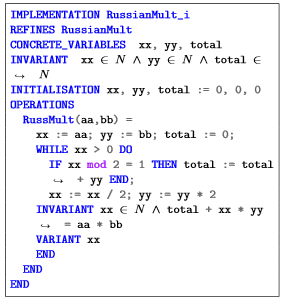
\includegraphics[width = \textwidth]{imagens/russianMult_i2.png}
\caption{Implementation. \cite{schneider2001b}}
\label{fig:russianMultImp}
\end{subfigure}
\end{minipage}
\begin{minipage}{0.45\textwidth}
\begin{subfigure}{\textwidth}
\centering
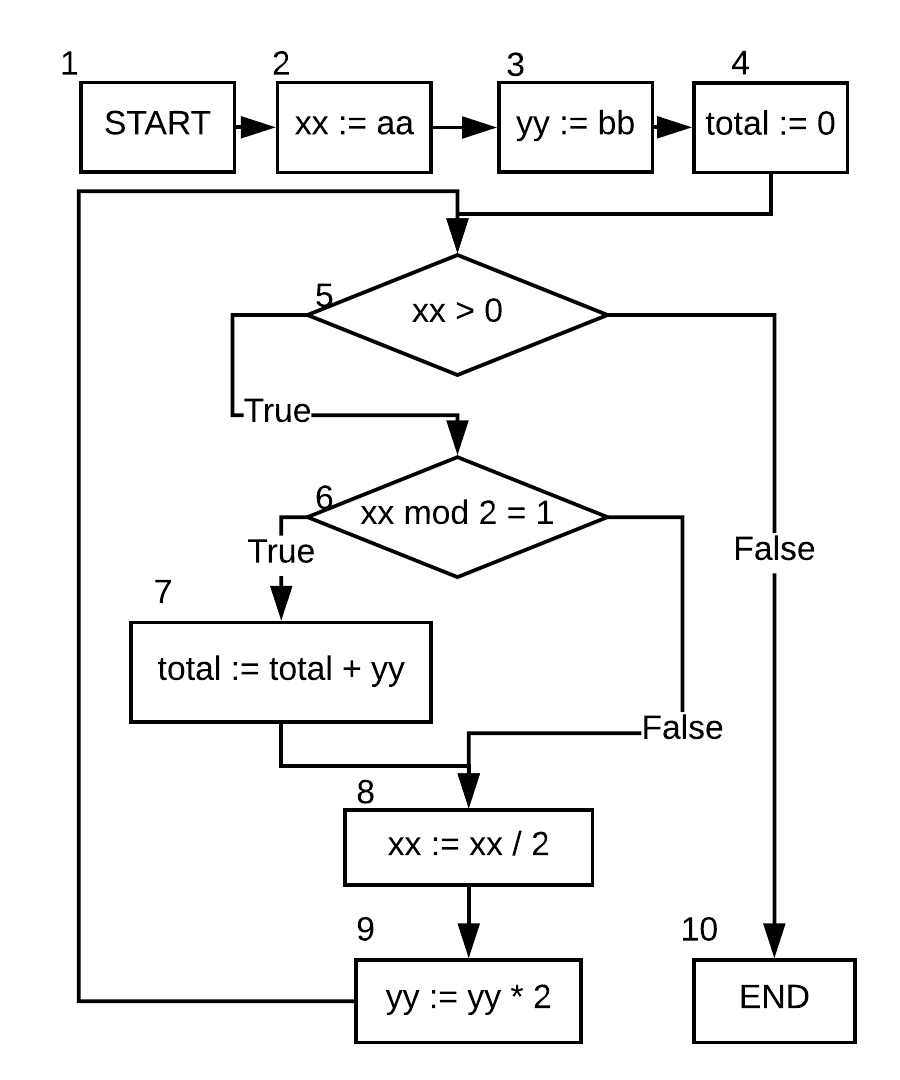
\includegraphics[width = \textwidth]{imagens/lacoGrafo.png}
\caption{Graph.}
\label{fig:russianMultGraph}
\end{subfigure}
\end{minipage}
\caption{Russia Multiplication Graph and Implementation.}
\end{figure*}

%Since the operation found in Figure \ref{fig:russianMultGraph} has a loop, it is possible to identify infinite paths and uncountable paths to test is not mechanically possible. 
Since the operation found in Figure \ref{fig:russianMultGraph} has a loop, it is possible to identify infinite paths. However, testing uncountable paths is not mechanically possible.
To bypass this situation, our tool does not compute all the paths. Instead of repeating the instructions inside the loop and generating different paths for each time the loop is executed, BTestBox counts the paths inside the loop just once and uses it to represent all the paths created with the repetition of the loop. We assume this because of the B method property - a loop always has to end, and this is defined in the clauses of the B method. Then, we define that BTestbox generates the following paths:

\begin{itemize}
    \item Path 1: 1, 2, 3, 4, 5, 6, 7, 8, 9, 5, 10.
    \item Path 2: 1, 2, 3, 4, 5, 6, 8, 9, 5, 10.
    \item Path 3: 1, 2, 3, 4, 5, 10.
\end{itemize}

\subsection{Writing Predicates} \label{writingPredicates}

During this section, we present how BTestBox uses the Hoare’s logic to create a predicate. Our tool relays on the Hoare Triple, with which it is possible to calculate how a command can change the state. 
This form of the Triple is the notation:

$$\{P\} C \{Q\}$$

\textit{P} represents the precondition for the execution of the command \textit{C}, and \textit{Q} is the post-condition established after the command. \textit{P} and \textit{Q} are states described in first-order logic. With those terms, it is possible to calculate the precondition by knowing the command and the post-condition. 

For writing the predicate, BTestBox does a bottom-up approach with Hoare's Logic. We chose this approach because of the B method property for proved implementations, which implies that a proved implementation always has to finish. Since it is possible to assume that the operation is going to end, the post-condition \textit{Q} is assumable true at the last statement ``END'' of a B operation.

%In order to generate the test cases, BTestBox writes the predicate related to each previous generated path of the model under test or until the chosen criteria is achieved. Even more, different criterion has separate goals, for example, with the PC is necessary to test every path and for the operation ``RussMult'' is necessary to test the three. Although, for ST if the path 1 is feasible, then just it need to be executed. Choosing the BC for the operation in the Figure \ref{fig:russianMultGraph}, the minimum necessary paths to be executed is two.

 BTestBox writes the predicate to generate the test cases. They are related to each previously generated path of the model that are under test. They remain under testing until the chosen criterion is achieved. Further more, the different criterion has separate goals, for example, with the PC criterion: it is necessary to test every path, and for the ``RussMult'' operation, it is needed to test all the three paths. However, for the ST criterion, if path 1 is feasible, only then, it will be executed. By choosing the BC criterion for the operation in Figure \ref{fig:russianMultGraph}, the minimum necessary paths to be executed is two.

The BTestBox procedure takes the path with the biggest amount of nodes to write the first predicate. Such consideration makes Path 1 the path under test. With the bottom-up approach, node 10 holds true and is the post-condition of the Hoare's Triple. Node 5 is the command. Since it needs to be a false guard, the value is the negative of the hold, generating the following scheme:

$$\{P\} C \{Q\} \implies \{P\} [\neg(xx > 0)] \{true\} \implies P: xx <= 0$$

After reaching node 5, since it is the guard of a loop, our tool divides the predicate into two: one partition for the inner part of the loop and the other for the outer part. The inner predicate is a post-condition indicating the values after running the loop and the outer is the previously calculated precondition for entering the loop. After calculating the inner predicate, both predicates are joined in a bigger predicate representing the post-condition of ending the operation. Then, BTestBox first calculates the predicate for the inner part, and the post-condition refreshes to hold true because the loops in B have to reach an end. Differently from node 5, node 9 is not a guard, so it can change the previously established variables, but since it is a new predicate and holds it true, nothing will change:

$$\{P\} C \{Q\} \implies \{P_i\} yy := yy * 2\{true\} \implies P_i: true$$

As it is possible to observe, the precondition remains the same as the post-condition. This happens because the variables in the statement do not manipulate the variables inside the post-condition and the command is not a guard. Such an effect occurs in the nodes 9,8,7. Reaching the sixth node, the triple changes into the following:

$$\{P\} C \{Q\} \implies \{P_i\} [xx\ mod\ 2=1]\{true\} \implies P_i: xx\ mod\ 2 = 1$$

When arriving at the guard of the loop, our tool joins the external and the internal calculated predicates. Therefore, it also assumes a quantification over the values that are modified inside the loop. And due to the B declarations, it wraps the values of the variables in the quantification over the invariant. This assures that the assumed values satisfy the proved B implementation. Finally, the precondition is:

$$P: \#(xx, yy, total).(xx > 0 \wedge xx\ mod\ 2 = 1 \wedge$$
$$ xx \in \mathbb{N} \wedge total + xx * yy = aa * bb) \wedge$$
$$\#(xx, yy, total).((xx \leq 0) \wedge xx \in \mathbb{N} \wedge total + xx * yy = aa * bb)$$

Then, BTestBox continues to walk through the path, but the quantification cannot be changed by statements that appear after it. Since there are no more guards until node 1, the predicate will remain the same. With node 1, the invariant of the abstract machine ``RussianMult'' and the precondition of the abstract operation are added in the predicate:

$$P: \#(xx, yy, total).(xx > 0 \wedge xx\ mod\ 2 = 1 \wedge$$
$$ xx \in \mathbb{N} \wedge total + xx * yy = aa * bb) \wedge$$
$$\#(xx, yy, total).(xx \leq 0 \wedge xx \in \mathbb{N} \wedge total + xx * yy = aa * bb) \wedge$$
$$xx : NAT \wedge yy : NAT \wedge total : NAT \wedge aa : NAT \wedge bb : NAT$$

Subsequently, it is necessary to solve the found predicate to assure that it is a valid predicate and has at least one solution. Our tool is not able to solve predicate and retrieve the possible inputs of an operation and its respective output, so we used the ProB constraint solver. The ProB returned that a possible solution is aa = 1, bb = 0, xx = 0, yy = 0, total = 0. That way, the inputs of a test case is defined.

Getting the outputs is a similar process, but instead of the post-condition of the end node being true, its foo variables equals each input variable. Then:

$$Q : foo\_aa = aa \wedge foo\_bb = bb \wedge foo\_xx = xx \wedge$$
$$foo\_yy = yy \wedge foo\_total = total$$

Writing a predicate and evaluating the outputs with the same process previously done returns the values foo\_aa = 1, foo\_bb = 0, foo\_xx = 0, foo\_yy = 0, foo\_total = 0. Finally, one test case is defined with the inputs and the expected outputs.

BTestBox continues the process. It does the same for paths 1 and 2. Similarly, the predicate for the inputs of the second path is:

$$P: \#(xx, yy, total).(xx > 0 \wedge \neg(xx\ mod\ 2 = 1) \wedge$$
$$ xx \in \mathbb{N} \wedge total + xx * yy = aa * bb) \wedge$$
$$\#(xx, yy, total).(xx \leq 0 \wedge xx \in \mathbb{N} \wedge total + xx * yy = aa * bb) \wedge$$
$$xx : NAT \wedge yy : NAT \wedge total : NAT \wedge aa : NAT \wedge bb : NAT$$

The next step is to call ProB and solve the predicate. The returned values for the inputs of the second path are aa = 2, bb = 0, xx = 0, yy = 0, total = 0. Identically, the outputs of path 2 are foo\_aa = 2, foo\_bb = 0, foo\_xx = 0, foo\_yy = 0, foo\_total = 0.

%After this procedure, BTestBox found the necessary test cases for achieving BC for the operation ``RussMult''. And they are shown in the table \ref{tab:TestCases}.
After this procedure, BTestBox found the necessary test cases for achieving the BC criterion for the ``RussMult'' operation, which are shown in Table \ref{tab:TestCases}.


\begin{table}[h]
\centering
\caption{Test cases for ``RussMult''}
\begin{tabular}{c|c|c|c|c|}
\cline{2-5}
                                & \multicolumn{2}{c|}{Test 1} & \multicolumn{2}{c|}{Test 2} \\ \hline
\multicolumn{1}{|c|}{Variables} & Input        & Output       & Input        & Output       \\ \hline
\multicolumn{1}{|c|}{aa}        & 1            & 1            & 2            & 2            \\ \hline
\multicolumn{1}{|c|}{bb}        & 0            & 0            & 0            & 0            \\ \hline
\multicolumn{1}{|c|}{xx}        & 0            & 0            & 0            & 0            \\ \hline
\multicolumn{1}{|c|}{yy}        & 0            & 0            & 0            & 0            \\ \hline
\multicolumn{1}{|c|}{total}     & 0            & 0            & 0            & 0            \\ \hline
\end{tabular}
\label{tab:TestCases}
\end{table}

\subsection{Creating Test Case Files}

In this section, we describe how BTestBox can manipulate the user files, insert ```get'' and ``set'' operations, and execute the test with the previously calculated inputs. 

Our tool copies the user files to keep the original B components and adds operations capable of changing the state of the variables. The ``set'' operation is responsible for setting the input values of variables that are defined and not used in the operation call. For the Russian multiplication implementation, the variables are xx, yy, and total. The ``get'' operations are responsible of providing the current state of each variable on the component. Every variable has a different ``get'' operation. Writing them to the model under test allows the BTestBox to check the state of the variables and it compares with the expected output that was previously calculated.

The test cases are defined based on the chosen coverage criteria. Different criterion will likely result in diverse test cases. BTestBox writes the test files capable of setting the test to a state defined in the test case in B. In a future process step, when the B files are translated to a computer language, all the test files are also translated using the same translator. The set test case has an operation for each test case scenario found during Section \ref{writingPredicates}. Such form allows it to test each test case in a different spot and makes it possible for the user to check when a failure is detected. Those operations call the operation under test with the inputs and create a auxiliary variable for storing and checking the values after the call. If the values are the same as expected, then the verdict ``true'' is returned, otherwise, the verdict is ``false''. Figure \ref{fig:SetTestModel} shows how the concrete set test operations are constructed.

% \begin{figure}
%     \centering
%     \begin{minipage}{0.46\textwidth}
%         \centering
        
%         \begin{minted}[frame=single,firstnumber=1,linenos=false,breaklines,fontsize=\small]{ocaml}
% OPERATIONS
%  verdict <-- TEST_1_RussMult =
%  BEGIN 
%   SetVarForTestRussMult(0,0,0);
%   VAR a1, a2, a3, a4, a5 IN
%   RussMult(1,0);
%   a1 <-- Get_xx; a2 <-- Get_yy;
%   a3 <-- Get_total;
%   a4 <-- Get_aa; a5 <-- Get_bb;
%   IF a1=0 AND a2=0 AND a3=0 AND
%       a4=1 AND a5=0 THEN
%     verdict := TRUE
%   ELSE verdict := FALSE END
%   END 
%  END;
%  verdict <-- TEST_2_RussMult =
%  BEGIN 
%   SetVarForTestRussMult(0,0,0);
%   VAR a1, a2, a3, a4, a5 IN
%   RussMult(2,0);
%   a1 <-- Get_xx; a2 <-- Get_yy;
%   a3 <-- Get_total;
%   a4 <-- Get_aa; a5 <-- Get_bb;
%   IF a1=0 AND a2=0 AND a3=0 AND
%       a4=2 AND a5=0 THEN
%     verdict := TRUE
%   ELSE verdict := FALSE END
%   END 
%                 \end{minted}
%         \caption{Concrete set test operations.}
%         \label{fig:SetTestModel}
%     \end{minipage}%
% \end{figure}

\begin{figure*}[ht]
\begin{minipage}{0.5\textwidth}
\begin{subfigure}{\textwidth}
\centering
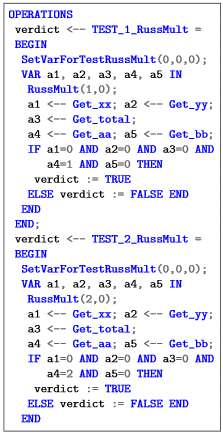
\includegraphics[width = \textwidth]{imagens/concreteSetTest.png}
\caption{Concrete set test operations.}
\label{fig:SetTestModel}
\end{subfigure}
\end{minipage}
\begin{subfigure}{0.49\textwidth}
\centering
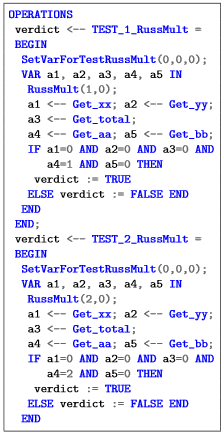
\includegraphics[width = \textwidth]{imagens/concreteRunTest.png}
\caption{Concrete run test operations.}
\label{fig:RunTestModel}
\end{subfigure}
\caption{Concrete test operations}
\end{figure*}

Once the B component for setting is written, our tool prepares another component capable of reading the answer of each test case operation. It can be found in Figure \ref{fig:RunTestModel}. The running of the test component implies in an approach to verify the B translator. Therefore, the user may have two possibilities of checking the compiler: the one automatically executed by BTestBox or animating the B component responsible for running the test.

% \begin{figure}
%     \centering
%     \begin{minipage}{0.45\textwidth}
%         \centering
%         \begin{minted}[frame=single,firstnumber=1,linenos=false,breaklines,fontsize=\small]{ocaml}
% LOCAL_OPERATIONS
%   verdict <-- Test_RussMult =
%     ANY kk WHERE kk : BOOL THEN verdict := kk END;
% OPERATIONS
%   verdict <-- Test_RussMult =
%   BEGIN
%     VAR a1, a2 IN
%       a1 <-- TEST_1_RussMult;
%       a2 <-- TEST_2_RussMult;
%       IF a1 = TRUE & a2 = TRUE THEN
%         verdict := TRUE
%       ELSE verdict := FALSE END
%     END
%   END;
%   verdict <-- Test_All =
%   BEGIN 
%     VAR v0 IN
%       v0 <-- Test_RussMult;
%       IF v0 = TRUE THEN
%         verdict := TRUE
%       ELSE verdict := FALSE END
%     END
%   END
%         \end{minted}
%         \caption{Concrete run test operations.}
%         \label{fig:RunTestModel}
%     \end{minipage}
% \end{figure}

In the BTestBox usual process, the next step is the translation of the code by a B compiler. While using a B translator, it is necessary to create a main file - BTestBox has the ability to write this piece of code. Finally, the code is translated, but it is not available for execution. Our tool also asks for a compiler, defined by the user, to create an executable file of the test. With the program of the test, it is possible to show the results of the execution in a new window for the user.

But that is not all: BTestBox also writes an HTML file that provides a summary of the test. It has three sections: The first page, Figure \ref{fig:report1}, shows the tested operations and the test results with the percentage of coverage; the second page, Figure \ref{fig:report2}, contains the inputs and expected outputs for every test, it also reports which objective was not successfully achieved; the third page, \ref{fig:report3}, presents the library with the links for all files used in the test: original files, test files, and translated files. 

\begin{figure*}[ht]
\begin{minipage}{0.45\textwidth}
\begin{subfigure}{\textwidth}
\centering
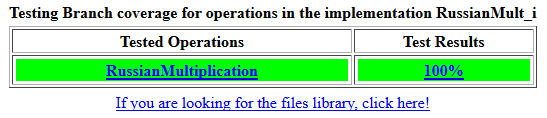
\includegraphics[natwidth=547,natheight=118,width = \textwidth]{imagens/reporte1.png}
\caption{First report page.}
\label{fig:report1}
\end{subfigure}
\begin{subfigure}{\textwidth}
\centering
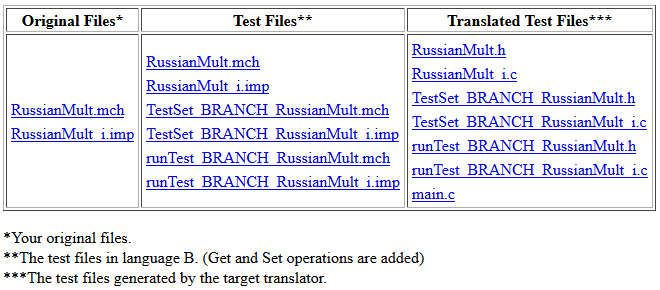
\includegraphics[natwidth=660,natheight=290,width = \textwidth]{imagens/reporte3.png}
\caption{Library report page.}
\label{fig:report3}
\end{subfigure}
\end{minipage}
\begin{subfigure}{0.50\textwidth}
\centering
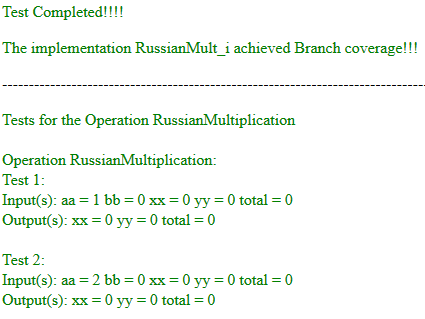
\includegraphics[natwidth=425,natheight=319,width = \textwidth]{imagens/reporte2.png}
\caption{Detailed report page.}
\label{fig:report2}
\end{subfigure}
\caption{Pages of the report}
\end{figure*}

\section{Results} \label{sec:Results}

%This section is responsible for discussing the results, the validation, and the potential improvements.

BTestBox was tested for a variety of different B clauses and structures, with the goal of assuring the correctness of the process and the functionality of the tool. Our tool ran more than 120 proved implementations presenting the B language. Additionally, one real B project granted by the \textit{ClearSy} enterprise was put under test.

The diverse components executed by our tool are exposed in Table \ref{tab:ValidationGroups}. The groups were divided regarding the language structure exercised with the B component.

\begin{table}[ht]
\centering
\caption{B Components Groups for validation.}
\begin{tabular}{l|c|}
\cline{2-2}
                                        & \multicolumn{1}{l|}{Quantity of implementations} \\ \hline
\multicolumn{1}{|l|}{Clauses}           & 14                                             \\ \hline
\multicolumn{1}{|l|}{Operation Call}    & 26                                             \\ \hline
\multicolumn{1}{|l|}{Depth one blocks} & 6                                              \\ \hline
\multicolumn{1}{|l|}{Depth two blocks} & 25                                             \\ \hline
\multicolumn{1}{|l|}{Depth three blocks} & 58                                             \\ \hline
\multicolumn{1}{|l|}{Industrial Confidential} & 1
\\ \hline
\end{tabular}
\label{tab:ValidationGroups}
\end{table}

\begin{itemize}
    %\item The clause group exercises the structures sees, extends, constants, constraints, imports, promotes, sets, variables, and local operations. Those elements are put in test in groups and separately to observe the changes in the predicate that each can perform.
    \item The "Clauses" group exercises the \underline{sees}, \underline{extends}, \underline{constants}, \underline{constraints}, \underline{imports}, \underline{promotes}, \underline{sets}, \underline{variables} and \underline{operations}. Those elements are tested both in groups and separately. Those tests observe the changes that each element can perform in the predicate.
    %\item Operation calls employ the operation calls in different contexts.
    \item The "Operation Call" employs operation calls in different contexts.
    %\item Depth blocks are sensitive to the instructions if-else, case, skip, while and assignment. They are grouped and nested to max depth of three. 
    \item "Depth" blocks are sensitive to the if-else, case, skip, while, and assignment instructions. They are grouped and nested to the maximum depth of three.
    %\item The industrial project is responsible for diverse contributions to BTestBox, with B structures non previous tested. Unfortunately, the tests generated for this case are very time consuming due the necessity of sets expansions.
    \item The "Industrial" project is responsible for different contributions to the BTestBox, with non-previously tested B structures. Unfortunately, the tests generated for this case are very time-consuming due to the necessity of set expansions.
\end{itemize}

All the presented implementation, excluding the industrial project, were exercised with all the coverage criteria supported by the BTestBox. Even contributing to the development of our tool, the industrial project was not able to fully test the project because of the time available.

Moreover, our tool was not implemented for the data structures of matrices and trees. In the current context, BTestBox can manipulate vectors. The current data structures and elements supported may be observed in Table \ref{tab:tabelaSuportados}.

\begin{table}[h]
\centering
\caption{Structures supported by BTestBox}
\label{tab:tabelaSuportados}
\begin{tabular}{|c|c|c|}
\hline
\multicolumn{2}{|c|}{Type}                     & Supports \\ \hline
\multicolumn{2}{|c|}{Arithmetic operators}   & $\surd$   \\ \hline
\multicolumn{2}{|c|}{Logical operators}       & $\surd$   \\ \hline
\multicolumn{2}{|c|}{Sets operators}  & $\surd$   \\ \hline
\multirow{3}{*}{Data structure} & Vectors  & $\surd$   \\ \cline{2-3} 
                                    & Matrices & X       \\ \cline{2-3} 
                                    & Trees  & X       \\ \hline
\end{tabular}
\end{table}

Our tool was also tested with the intention of expliciting the problems of using the \textit{ProB} tool and the scalability of BTestBox. To present that, giant B implementations were analysed and metrics were registered. A variety of lexical elements of the B language were created at random with nested instructions. They were designed to test the scalability of a B translator to LLVM \cite{deharbebtestbox}. Those files may be classified by the size of the operations: the variables that define the generation of the files are the number of nesting in command block and the quantity of blocks inside an operation. Such operations can be built around 1, 10, 50, 100 or 500 blocks and the nesting level varies between 1 and 5.

%For the scalability tests, was used a computer with the operating system Windows 10 64 bits, with a processor Intel Core i5\-6300HQ 2300 GHz and 8 GB de memória RAM. We observed that the scalability may stick to minor size implementations since the Atelier-B, version 4.3.1, available on the computer does not generate the proof obligations and the BXML tree file necessary for BTestBox.
We \textcolor{blue}{initially} used a computer with the Windows 10 64 bits operating system, with an Intel Core i56300HQ 2300 GHz processor and 8 GB of RAM for the scalability tests. %We observed that the scalability might stick to a minor size implementations since the Atelier-B, version 4.3.1, available on the computer does not generate the proof obligations and the BXML tree files which are required for BTestBox.

 
To improve the results, we researched and implemented threads inside the tool.
This way, BTestBox can execute its procedure to various operations of the same implementation and the evaluation with ProB occurs at the same time for all. This severally reduce the time for the predicate evaluation. In Table \ref{tab:escalabilidadeSuper}, it is possible to observe the results of tests using a computer with 2 CPUs Intel Xeon Sixteen-Core E5-2698v3 allocating in the maximum 20 cores with 80 Gigabytes of RAM, the time was reduced approximaletly in 90\%.
All examples of table \ref{tab:escalabilidadeSuper} can be executed in a cloud computer costing less than one US dollar.


Additionally, the implementation provided in \cite{deharbebtestbox} had to be adapted to be properly used with BTestBox, but it did not lose any nesting or instruction. Such adaptations are needed because the implementations are not proved. They present decisions that perform mathematical calculus without a solution. Also, they have operation calls. In the current state, our tool is not able to manage operation calls due to the necessity of using a close Atelier-B function that was only available during the process of validation.

During the process of testing, it is notorious that the time for evaluation is longer than the other steps of BTestBox. The results are shown in Table \ref{tab:escalabilidade}. It is possible to observe the amount of time spent for the evaluation with ProB.

\begin{table}[h!]
\centering
\caption{Implementations for scalability}
\label{tab:escalabilidade}
\begin{tabular}{|c|c|c|c|}
\hline
Component                                                                                          & COMP\_1seq1 & COMP\_2seq1 & COMP\_3seq1 \\ \hline
\begin{tabular}[c]{@{}c@{}}Quantity of\\ operations\end{tabular}                                    & 39          & 199         & 999         \\ \hline
Nesting level                                                                                          & 1           & 2           & 3           \\ \hline
\begin{tabular}[c]{@{}c@{}}Commands\\ by block\end{tabular}                                         & 1           & 1           & 1           \\ \hline
\begin{tabular}[c]{@{}c@{}}Execution time\\ (seconds)\end{tabular}                       & 587.36      & 3102.89     & 18214.17    \\ \hline
\begin{tabular}[c]{@{}c@{}}Predicate\\ evaluation time\\(seconds)\end{tabular} & 525.63      & 2858.76     & 15274.43    \\ \hline
\begin{tabular}[c]{@{}c@{}}Time spent\\ for evaluation (\%)\end{tabular}   & 89.49       & 92.13       & 83.86       \\ \hline
\end{tabular}
\end{table}

For some operations, such as the component with operations of 2 nested instructions in 10 blocks, the number of paths calculated were over 750,000. Since the B implementations are generated at random, most of the paths are unfeasible. This case shows that the time for evaluation is a problem, but it is also possible to infer that picking a better method for choosing the tested path will drastically reduce the time of BTestBox execution. In Table \ref{tab:escalabilidadeComp2}, it is possible to notice that the evaluation time can take more than 16 days. 

\begin{table*}[h!]
\centering
\caption{Scalability test for the COMP\_2seq10 implementation}
\label{tab:escalabilidadeComp2}
\resizebox{\textwidth}{!}{%
\begin{tabular}{|c|c|c|c|c|c|}
\hline
Component                     & Operation & Quantity of Paths & \begin{tabular}[c]{@{}c@{}}Total execution \\ time (seconds)\end{tabular} & \begin{tabular}[c]{@{}c@{}}Predicate evaluation\\  time (seconds)\end{tabular} & \begin{tabular}[c]{@{}c@{}}Time spent \\ for evaluation (\%)\end{tabular} \\ \hline
\multirow{3}{*}{COMP\_2seq10} & ID00000   & 4320              & 8637.51                                                                   & 7647.99                                                                        & 88.54                                                                     \\ \cline{2-6} 
                              & ID00001   & 87480             & 205552.43                                                                 & 168452.96                                                                      & 81.95                                                                     \\ \cline{2-6} 
                              & ID00002   & 787320            & 1781627.72                                                                & 1423590.45                                                                     & 79.90                                                                     \\ \hline
\end{tabular}}
\end{table*}



\begin{table}[h]
\centering
\caption{Scalability test with the supercomputer}
\label{tab:escalabilidadeSuper}
\resizebox{0.6\textwidth}{!}{%
\begin{tabular}{|c|c|c|c|}
\hline
Component                                                                        & Comp1\_Seq1 & Comp2\_Seq1 & Comp3\_Seq1 \\ \hline
\begin{tabular}[c]{@{}c@{}}Execution time\\ without\\ supercomputer\end{tabular} & 587,36 s    & 3102,89 s   & 18215,17 s  \\ \hline
\begin{tabular}[c]{@{}c@{}}Execution time\\ with \\ supercomputer\end{tabular}   & 38,08 s     & 176,91 s    & 2286,42 s   \\ \hline
\begin{tabular}[c]{@{}c@{}}Time reduced\\ for evaluation\end{tabular}            & 93,52\%     & 94,30\%     & 87,45\%     \\ \hline
\end{tabular}%
}
\end{table}

% \begin{table}[h!]
% \centering
% \caption{Scalability test for COMP\_2seq10}
% \label{tab:escalabilidadeComp2}
% \begin{tabular}{|c|c|c|c|}
% \hline
% Component                                                                      & \multicolumn{3}{c|}{COMP\_2seq10} \\ \hline
% Operation                                                                      & ID00000  & ID00001   & ID00002    \\ \hline
% Quantity of paths                                                              & 4320     & 87480     & 787320     \\ \hline
% Total execution time                                                           & 8637.51  & 205552.43 & 1781627.72 \\ \hline
% \begin{tabular}[c]{@{}c@{}}Predicate evaluation\\  time (seconds)\end{tabular} & 7647.99  & 168452.96 & 1423590.45 \\ \hline
% \begin{tabular}[c]{@{}c@{}}Time spent for\\  evaluation (\%)\end{tabular}      & 88.54    & 81.95     & 79.90      \\ \hline
% \end{tabular}
% \end{table}

\section{Potential Improvements}


\marginpar{Recentes melhorias compatível com os sistemas operacionais Windows, Linux e OsX. Adição de threads e configuração para execução em servidor dedicado. }

In this Section we relate the possible points of improvements of the BTestBox. All the mentioned improvements are planned and will be in the authors' future work.

In the current state, our tool supports five coverage criteria, and our study aims to add the Modified Condition/Decision Coverage (MC/DC). Since the Combinatorial Coverage is stronger than the MC/DC, our tool is already capable of generating tests that will achieve the MC/DC, but CoC is more time consuming since it demands more tests. It is possible to satisfy MC/DC without achieving CoC.

Currently, BTestBox is only able to test the C compiler, the C4B with different translation profiles, and to use the compiler GCC, but it has plenty of space for development and with small improvements, it can include other B translators such as LLVM and ADA with the user of a correspondent compiler for executing the translated code. %The tool is also only available for Windows, but we plan to diffuse it for the Mac and Linux OS.

A problem happens when there is a machine that does not have an implementation. Usually, this is the case of base machines, and this limits the number of real projects which BTestBox could be applied for. \marginpar{Isso não é um problema do BTestBox. Isto é uma limitação de qualquer gerador de testes baseados em modelos/especificação de software, conceitualmente não há como resolver, apenas informar ao usuário.} 
To accomplish that, BTestBox has to deal with non-deterministic predicates. The procedure gets complicated when the tool is trying to test an implementation and wants to compare whether the output is the same as to when the ProB evaluates the predicate. BTestBox only accepts deterministic machines or implementations because we focus on deterministic tests.

\section{Threats to Validity}

Despite our efforts and the measures taken throughout our work to assure the functionality of our tool and the validity of our results, our study faces some threats to validity. Also, the validation of our tool faces limitations that may impact on the external validity.

External validity alludes to the degree to which our experiments' results can be generalised. The most relevant and potential threat to the validity of BTestBox is the population of the models tested with our tool. Since the models developed for testing BTestBox are limited and made during the proper creation of our tool, it is not possible to assure the full correctness. Additionally, even concerning the number of tests, the tool needs maturation and to be operated by more users with different cases and situations.\marginpar{Desnecessário: ''the tool needs maturation and to be operated by more users with different cases and situations''}. Notwithstanding, related to the external validity, there is the necessity of employing a third party function that is not available in the regular distribution of the third party tool.

%To address these potential threats, more studies will be expanded by the authors using a bigger range of models and a more powerful computer, reducing the time of tests and expanding the quantity number of models tested by BTestBox.

\section{Related Work} \label{sec:RelatedWork}

Generating test cases from models is a subject that has been studied by research groups for several years. The work \cite{shafique2010systematic} contains an interesting systematic review about testing a software system by using a test model of its behaviour, and it was useful to BTestBox.

Another important work is in \cite{marinescu:2015}. Its authors showed a new overview of the current state of the art for model-based testing tools that use requirement-based specification languages. They quoted two tools compatible with the B method: ProTest \cite{leuschel:2005} and BZ-TT \cite{bouquet:2002}.

The BZ-TT contains an environment for boundary-value test generation from Z and B specifications. This tool relies on constraint solving, and its goal is to test every operation of the system at every reachable boundary state. A boundary state is a system state in which at least one of the state variables has a maximum or minimum boundary value. It is not open source, and its last public news was in the year of 2003.

ProB is another tool with support to generate tests from B models. It has an automatic test environment for B specifications and a component called ProTest.
Its component uses model-checking techniques to find test sequences that satisfy its test generation parameters. The user has to define the requirements to be satisfied by the test cases. These requirements are operations that must be covered and predicates that must hold true at the end of each test case. The tool only generates abstract test cases that have to be implemented before they can be executed. BTestBox is capable of generating executable test scripts. That is an advantage. Another recent contribution to this research field is the BETA tool \cite{ernesto_thesis:2016}. 

The BETA generates test code using input space partitioning and logical coverage criteria. It also automates the generation tests and supports several coverage criteria. The generated tests are based on abstract B models, and some important information about the model are ignored.
Information ignored by BETA may generate inaccurate tests related to the B concrete model. Differently, BTestBox generates test cases directly from B concrete model which is a closer representation of the software.
Another relevant difference is that BETA is focused on unit testing, while BTestBox tests both approaches on unit testing and the entire module. Furthermore, BTestBox has previous experiments with massive and random tests \cite{deharbebtestbox}.

\section{Conclusions and Future Work} \label{sec:Conclusion}

Currently, BTestBox is a free and open-source tool under Berkeley-licensed software.
This tool was born from an international collaboration between the academia and the software industry. The collaboration resulted in an initial version of the tool. Now, the goal is to increase the maturity of BTestBox to deal with industrial applications.
The developed software is maturing and the tool offers an important contribution to the community.

Several components were created with different B structures to test the functionality and correctness of the BTestBox. More than 120 B concrete models were created to test the B language, and one model, simulating a real used B program, was provided by \textit{ClearSy}.

BTestBox is already capable of generating tests that verify MC/DC. Our tool is capable of generating tests to verify the Combinatorial Coverage, since it demands the test of all possible combinations of guards, achieving CoC implies in being successful at MC/DC. Unfortunately, CoC generates a high number of tests. Efforts are concentrated in developing an approach to generate fewer test cases and achieve the required coverage.

BTestBox's future research has to be towards improving the performance. This is a problem since it calls ProB and sometimes the model checker has to expand a big set or various sets. The time to run a predicate with many clauses is enormous in comparison with predicates without any expansion. To solve this, the predicate generated by BTestBox has to be simplified with only the conditions that are bound to the variables that are used in operation.

When considering the evaluation of the predicate, BTestBox inherits every limitation from the logic expression solver (ProB). There are other candidate solvers that help to minimise the restrictions, and they will be studied.

Since BTestBox uses B translators, if the translator has any limitation to B language, it is also applied to our tool. However, there are several B translators, and the BTestBox's approach is compatible with all of them. 

We developed an approach using threads that decreased the time for running one implementation with more than one operation. This cut the time needed for solving operations, using a computer with sufficient cores for running all the operations, the time of execution is bounded to the most expensive operation. This is an improvement that made the execution of big implementations ten times faster.

\section*{Acknowledgement}
  The authors would like to especially thank ClearSy System Engineering for providing the industrial case and support. 

  The authors would also like to thank the anonymous referees for their valuable comments and helpful suggestions. 
  
  The work is supported by the Federal Institute of the Rio Grande do Norte, the Federal University of Rio Grande do Norte and CAPES (Coordination of Improvement of Higher Level Personnel).
  This work was grammatically reviewed by Antonio Henrique Nepomuceno Coelho (Federal English Teacher at IFRN).



%
% ---- Bibliography ----
%
% BibTeX users should specify bibliography style 'splncs04'.
% References will then be sorted and formatted in the correct style.
%

\bibliographystyle{splncs04}


\bibliography{bibs} 

\end{document}
